%!TEX program = xelatex

\documentclass[a4paper,11pt]{article}

% Paquetes necesarios
%\usepackage[utf8]{inputenc}
\usepackage[spanish]{babel}
\usepackage{amsmath, amssymb}
\usepackage{graphicx} % Paquete para manejar imágenes
\usepackage{fancyhdr}
\usepackage{hyperref}
\usepackage{lipsum}
\usepackage{tocbibind}
\usepackage{geometry}
\geometry{left=3cm,right=2.5cm,top=2cm,bottom=2cm}
\usepackage{float}
\usepackage{fontspec}
\usepackage{caption}
\setmainfont{Times New Roman}

% Configuración del pie de página
\pagestyle{fancy}
\fancyhf{}
\fancyfoot[C]{\thepage}

\begin{document}
% portada
\begin{titlepage}
    \begin{center}
        \vspace*{1cm} 
        
\includegraphics[width=1\textwidth]{./images/uc3m.jpg}
        
        \vspace*{3cm} 
        
        {\LARGE Criptografía y seguridad informática\\[0.5cm]} 
        {\LARGE G24 - Entregable 2 \\[0.5cm]}
        
        \vspace*{6cm}
        
        \textbf{Javier Martín Pizarro: 100495861@alumnos.uc3m.es} \\[0.5cm]
        \textbf{Alberto Pascau Sáez: 100495775@alumnos.uc3m.es} \\[0.5cm]
        \textbf{Raúl Armas Seriña: 100495746@alumnos.uc3m.es} \\[0.5cm]
        
        \vspace*{3cm}
        \textbf{GitHub:
        \href{https://github.com/Albrtito/CriptCript.git}{Albrtito/CriptCript.git}}\\[0.5cm]

    \end{center}
\end{titlepage}

% Eliminamos el índice de contenidos
\tableofcontents
\vspace{2cm}
%\newpage


% Introducción sin numeración de capítulo
\section{Propósito de la aplicación. Estructura interna}

\subsection{Propósito de la aplicación}

La aplicación simula una página web, levantada en local por el propio usuario,
en la que se pueden crear desafíos criptográficos(\textit{challenges}) con algoritmos de cifrado
clásico.\\\\
A la hora de crear un desafío cada usuario podrá elegir el algoritmo con el que
cifrar su desafío.El objetivo de otros usuarios será resolver que algoritmo de
cifrado se ha utilizado y el valor de la clave del cifrado; para ayudar en el
descifrado de desafíos la applicación implementará herramientas de
criptoanálisis simples.\\
Cada desafío sera público o privado, dependiendo de la elección que haga su
autor en su creación.
\begin{itemize}
    \item \textbf{Desafío público:} cualquier usuario registrado tiene acceso a ellos.
    \item \textbf{Desafío privado:} solamente pueden ser compartidos con un
        único usuario. El creador del desafío selecciona qué usuario será capaz de verlo.
\end{itemize}

El propósito de esta aplicación es generar un sistema informático que cumpla
unos requisitos mínimos. Nótese que a medida que la práctica avance, esta lista
podrá verse modificada. Los requisitos para esta primera entregá incluyen las
necesidades mínimas de la práctica.
son:\begin{enumerate}
    \item El sistema debe de ser capaz de registrar y autenticar usuarios.
        Guardando su información confidencial correctamente cifrada(contraseñas).$\rightarrow$\textbf{Requisito de confidencialidad}
    \item El sistema debe ser capaz de permitir un inicio de sesión donde se sea capaz de obtener y comparar 
        los datos cifrados de los usuarios de la base de datos con los proporcionados por el cliente.
    \item El sistema debe de ser capaz de guardar y recuperar desafíos usando
        cifrado simétrico/asimétrico. 
        $\rightarrow$ \textbf{Requisito de confidencialidad}
    \item El sistema debe de ser capaz de permitir a un usuario $A$ leer el desafío creado por el usuario $B$ si este se lo ha compartido.
    \item El sistema debe de autenticar que los mensajes mandados por usuarios a la
        base de datos no han sido alterados y son de quien dicen ser $\rightarrow$ \textbf{Requisito de Integridad y
        Autenticidad}
    \item Para cumplir con el requisito 5 el sistema ha de implementar alguna
        forma de MAC o cifrado autenticado
    \item El sistema debe de ser capaz de mostrar en pantalla todos los
        desafíos, privados y públicos, específicos para cada usuario.
    \item Para cada usuario registrado, el sistema debe de crear un certificado emitido por una entidad $ADMIN$.
    \item Para cada mensaje, debe de crearse una firma digital que verifique que el mensaje 
        no ha sido modificado por terceros. $\rightarrow$ \textbf{Requisito de Integridad y Autenticidad}
\end{enumerate}

\subsection{Estructura interna}

Esta aplicación consta de tres partes fundamentales:
\begin{itemize}
    \item \textbf{Frontend:} esencial para la experiencia de usuario. Actua como interfaz entre el cliente y el backend.
    \item \textbf{Backend:} donde se encuentra la API, implementada usando
        Flask. Todos los mecanismos de cifrado, autenticación y \textit{hasheo} se encuentran en este directorio.
    \item \textbf{Base de datos:} creada usando MariaDB SQL debido a su
        simplicidad. Actualmente la base de datos utiliza 3 bases de datos:
        mensajes, firma digital y certificados. De esta manera simulamos un entorno lo más independiente
        posible respecto al resto, aumentando la seguridad de nuestra aplicación. Puede ver un ejemplo en el
        \hyperref[sec:TablasSQL]{primer anexo}. 
\end{itemize}
La base del backend y de la base de datos han sido tomadas desde el repositorio
Open Source \textbf{backend-builderplate} del alumno y participante en esta
práctica Javier Martín, una iniciativa que permite agilizar y automatizar el
proceso de levantar una API y una base de datos que complemente a una interfaz
de usuario. La estructura del código de este proyecto hereda del repositorio original.%
\footnote{Repositorio original:
\url{https://github.com/jmartinpizarro/backend-builderplate}.}\\

\textbf{El uso de cada parte y su inizialización usando docker se recoge en el
archivo $README.md$ del repositorio, así como una explicación similar a esta de
la estructura del proyecto.}\\

\subsubsection{Frontend}
La carpeta del frontend contiene todo lo relacionado con la visualización de la
web, `html`, `css`, `javascript`. Los estilos (css) y scripts(Javascripts)
tienen sus propias subcarpetas, el html se encuentra directamente bajo la
carpeta frontend debido a que son pocos archivos y es ahí donde se inicializa el
servidor del frontend. \\

Actualmente no hay protección frente a un ataque de búsqueda de urls, cualquiera puede acceder a todo el contenido de la carpeta frontend desde la web.

\subsubsection{Backend}
La carpeta del backend contiene los archivos de `app.py` y `requirements.txt` que recogen la creación de la api e instalación de los requisitos necesarios en el servidor de backend. El resto del código se encuentra bajo src. Aquí diferenciamos entre tres carpetas:
\begin{itemize}
\item \textbf{mariaDB} $\rightarrow$ Métodos relacionados con la conexión a la DB

\item \textbf{utils} $\rightarrow$ Clases ocupadas de la autenticación, encriptación, generación de claves y hasheado, además del manager ocupado de utilizar todas esas clases para cifrar/descifrar y autenticar mensajes `MessageManager.py`. La clase que conforma la firma digital y las funciones de certificados también se pueden encontrar aquí.

\item \textbf{unittest} $\rightarrow$ Collección de test para comprobar que
    todas las clases funcionan correctamente. Actualmente solo se han
    implementado test para el HMAC pero se establecerá como objetivo para la
    segunda entrega crear test para el resto de clases.

\item \textbf{routes} $\rightarrow$ colección de rutas estáticas para la API de 
    Flask con la que realizaremos ciertas funciones dependiendo de las acciones que
    realice el usuario desde la interfaz.
    
\end{itemize}

De estas cuatro carpetas utils es la que interesa para evaluar los métodos
criptográficos implementados. Esta carpeta se ha divido según el propósito del
algoritmo que representa cada clase, creando secciones para algoritmos de
\textbf{autenticación, encriptación, generación de claves, cifrado autenticado, generación y verificación de hashes y
cifrados cásicos, firma digital y certificados}. \\

\begin{itemize}
    \item \textbf{Todos estos algoritmos criptográficos han sido implementados usando la librería de python cryptography}
\end{itemize}

\vspace{0.5cm}
\fbox{
    \begin{minipage}[t]{0.8\textwidth}
        \textbf{NOTA:} Para esta entrega solo se utilizan algoritmos de cifrado simétrico como AES y cifrado asimétrico como RSA (ya que es el estándar frente a DSA). En general, el sistema usa un cifrado híbrido que añade un extra de seguridad a los protocolos usados.\\
        También usaremos RSA para firma digital y certificación, además de HMACs para aportar integridad a los mensajes de los usuarios.
    \end{minipage}
}

\subsection{Flujo de código}
\textbf{A fecha de la entrega final encontramos el siguiente flujo en el código de la aplicación:} 
\begin{itemize}
    \item Inicializamos las bases de datos con el certificado ADMIN (autoridad certificadora), usuario y contraseña y claves para la firma digital.
    \item Cuando el usuario se registra, se crea un usuario y una contraseña correctamente hasheada, además de sus claves de firma y un certificado firmado por la entidad ADMIN (autoridad certificadora).
    \item En la creación de mensajes, se cifra el contenido y también se firma para poder comprobar la integridad (y autenticidad) más adelante.
    \item A la hora de renderizar los mensajes, comprobamos que la clave pública del usuario que creó el mensaje se verifique con su certificado, que la firma del mensaje sea la correcta y por último desciframos (no sin antes comprobar si el HMAC es el correcto).
\end{itemize}

\subsubsection{Flujo de código: Usuario crea un mensaje privado}

Asumimos que el usuario $A$ ya ha sido creado y ha iniciado sesión. Ha creado un mensaje privado a un usuario $B$. El siguiente diagrama describe el flujo del código ejecutado para cifrar el mensaje, generar una firma digital y el resto de lógica en lo que respecta a la criptografía:

\section{Firma Digital}
\label{sec:firmaDigital}
La firma digital es usada para verificar la integridad y autenticidad de los mensajes que los usuarios han creado y que se van a renderizar. 

Inicializamos una base de datos separada a la anterior (donde almacenábamos la información de los usuarios y los mensajes), simulando un provedor externo e independiente. 

Para la firma, se usa el algoritmo RSA. Se pensó en usar DSA, pero ya que RSA es el estándar de la industria, el código ha sido diseñado para ser lo más verídico posible respecto a la realidad.

En esta base de datos, llamada \textit{digital\_firm}, existen dos tablas distintas:
\begin{itemize}
    \item secure\_keys\:encargada de almacenar una clave pública y una clave privada cifrada para cada usuario (totalmente independientes a otras bases de datos)
    \item digital\_signatures\: la firma digital generada por cada mensaje que ha creado un usuario
\end{itemize}

Para ello recogemos tres funciones en el archivo \textit{DigitalSignManager.py}:
\begin{itemize}
    \item generate\_rsa\_keys()\: generamos un par de claves relacionadas entre ellas: una clave pública y una clave privada en formato PEM binario.
    \item create\_signature(): dada una clave privada PEM y un mensaje, firmamos dicho mensaje.
    \item verify\_signature(): dada una clave pública PEM, un mensaje y una firma, comprobamos si dicha firma es verdadera o no.
\end{itemize}

De nuevo, mantenemos una estructura lo más modular posible, intentando seguir un estándar apropiado para el correcto entendimiento del código. 

Si bien las funciones no tienen ningún \textit{log} cuando son definidas, en otras partes del código donde son invocadas sí que se hace un \textit{log} para enseñar los valores obtenidos.

Firma digital es usada especialmente en la renderización de mensajes, ya que al hacer una \textit{query} a la base de datos, obtenemos una lista con todas las filas disponibles. 

Para cada mensaje, comprobamos si la firma que se relaciona con ese mensaje es la misma que la que nosotros generamos. Si no es así, enviaremos un mensaje en la terminal diciendo que dicho mensaje no se verifica correctamente, y que por lo tanto ha sido eliminado de la lista de renderizado (el usuario al que iba dirigido no podrá verlo).

\section{Certificados}
\label{sec:certificados}

Los certificados son usados ampliamente en la industria para comprobar datos y aportar autenticidad e integridad a mensajes o interacciones con el sistema.

En este proyecto, también se ha implementado una jerarquía de entidades certificadoras para poder realizar estas acciones correctamente. La jerarquía es la siguiente:

\begin{figure}[h]
    \centering
    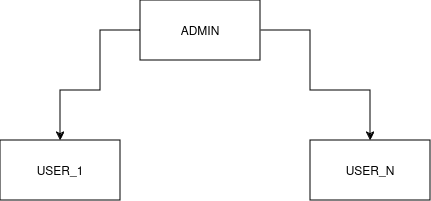
\includegraphics[width=0.6\textwidth]{./images/certificatesStructure.png}
    \caption{Jerarquía de entidades certificadoras}
    \label{fig:jerarquia}
\end{figure}

La entidad certificadora \textbf{ADMIN} es generada en la inicialización del proyecto. Para ello, tenemos una base de datos totalmente inpendiente que se encarga de guardar los certificados creados.

El certificado de esta entidad es firmado por sí misma, por lo que el usuario asume que es una entidad verífica y confiable.

Estos certificados son usados para verificar que la clave pública que se usa en firma digital es efectivamente la clave oficial de un usuario, y no una clave que pueda suponer un ataque a confidencialidad o veracidad de la información.

Para cada usuario que se registra en la aplicación se genera un certificado que es firmado por la entidad emisora \textbf{ADMIN}. Se guarda la clave pública generada para la firma como clave pública del certificado.

Antes de renderizar cada mensaje, comprobamos que el certificado es correcto y que la información es la correcta. Tras esto, procedemos con el flujo previamente mencionado (firma digital, descifrado, \textit{response}). 

Si la información del certificado obtenido no es correcta (es decir, que la verificación falla), eliminamos el mensaje de la lista de renderizado y emitimos un \textit{log} en la terminal para que quede constancia del error que ha ocurrido en la verificación.
\end{document}
